\documentclass[12pt,a4paper]{article}
\usepackage[utf8]{inputenc}
\usepackage[spanish]{babel}
\usepackage{amsmath}
\usepackage{graphicx}
\usepackage{geometry}
\usepackage{float}
\usepackage{caption}
\usepackage{booktabs}
\usepackage{enumitem}
\usepackage{hyperref}
\usepackage{comment}

\geometry{a4paper, margin=1in}
\hypersetup{
    colorlinks=true,
    linkcolor=blue,
    filecolor=magenta,      
    urlcolor=cyan,
}

\renewcommand{\figurename}{FIG.}
\renewcommand{\tablename}{TABLA}

\begin{document}

\begin{center}
    \huge\textbf{PRÁCTICA 2} \\
    \vspace{0.5cm}
    \huge\textbf{CARACTERÍSTICAS DEL DIODO ZENER}
\end{center}

\section*{Objetivos}
\begin{enumerate}
    \item Medir los efectos de las polarizaciones directa e inversa sobre la corriente en un diodo zener.
    \item Determinar y representar gráficamente la característica tensión-corriente de un diodo zener.
    \item Construir un regulador de tensión zener y determinar experimentalmente el margen en el cual el zener mantiene una tensión constante de salida.
\end{enumerate}

\section*{Información Preliminar}

\subsection*{Funcionamiento del diodo zener}

Las características de un diodo de estado sólido dependen del material semiconductor con el cual está construido el diodo, de la naturaleza y extensión del «dopado» de este material y de la construcción y dimensiones del dispositivo.

El diodo semiconductor se ha estudiado en la Práctica 1 y funciona dentro de su característica de corriente de polarización directa. Hay cierta clase de diodos llamados diodos zener cuyas características peculiares de corriente y tensión con polarización inversa hacen posibles aplicaciones completamente diferentes que las que tiene el diodo de cristal. El símbolo de un diodo zener está representado en la figura~\ref{fig:simbolo_zener}.

\begin{figure}[H]
    \centering
    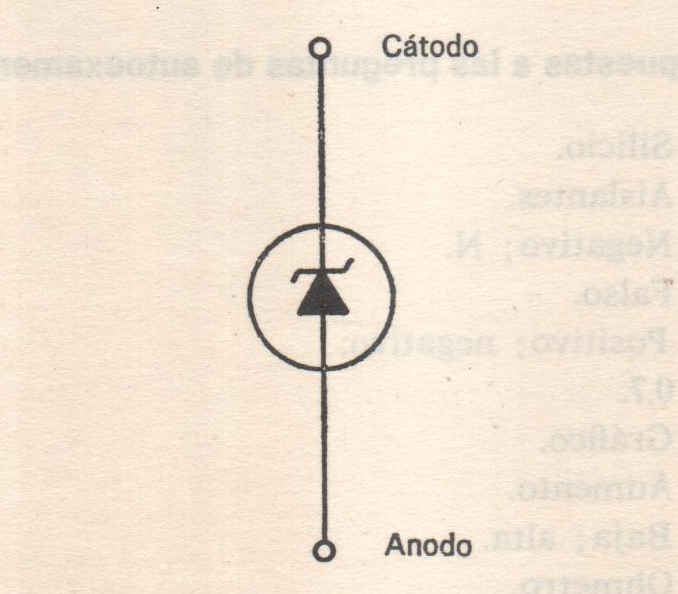
\includegraphics[width=0.3\textwidth]{simbolo_zener.png}
    \caption{Símbolo de un diodo zener.}
    \label{fig:simbolo_zener}
\end{figure}

La figura~\ref{fig:caracteristica_zener} es el gráfico de la característica típica tensión-corriente de un diodo zener. Cuando el diodo está polarizado en sentido directo actúa como un interruptor cerrado y la corriente directa aumenta con la tensión aplicada. La intensidad de la corriente directa está limitada por los parámetros del circuito. Cuando el diodo está polarizado en sentido inverso fluye una pequeña corriente inversa $I_S$, llamada corriente de saturación. $I_S$ permanece relativamente constante a pesar de que aumente la polarización inversa, hasta que se alcanza la región disruptiva zener, en la vecindad de la tensión zener $V_Z$. En esta condición la corriente inversa comienza a aumentar rápidamente a causa del efecto de avalancha. Finalmente, la ruptura zener (un brusco aumento de la corriente) tiene lugar cuando se alcanza la tensión zener $V_Z$.

\begin{figure}[H]
    \centering
    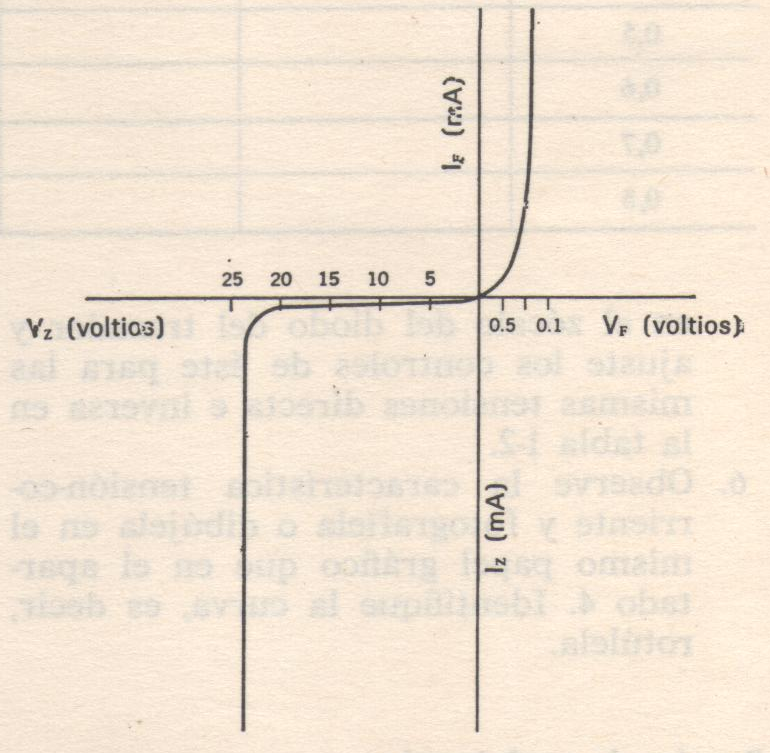
\includegraphics[width=0.6\textwidth]{caracteristica_zener.png}
    \caption{Característica de diodo zener.}
    \label{fig:caracteristica_zener}
\end{figure}

En esta región, pequeñas variaciones de la tensión dan lugar a grandes cambios de la corriente. Evidentemente, hay grandes variaciones de la resistencia efectiva de la unión PN en esta región.

La ruptura zener no da lugar necesariamente a la destrucción del diodo. Mientras la corriente que pasa por el diodo esté limitada por el circuito externo a un nivel que esté dentro de su capacidad de potencia, el diodo funciona normalmente. Por otra parte, reduciendo la polarización inversa por debajo de la tensión zener, se puede hacer que el diodo funcione fuera de su nivel de ruptura y vuelva al nivel de la corriente de saturación.

El proceso mediante el cual se conmuta el diodo entre sus estados de corriente zener y de corriente no zener se puede repetir reiteradamente sin que se deteriore el diodo. Sin embargo, obsérvese que hay un cierto retardo de tiempo, llamado tiempo de recuperación, en la conmutación del diodo de uno a otro estado.

\subsection*{Especificaciones}
Los fabricantes facilitan una hoja de especificaciones con cada tipo de diodo zener. Las especificaciones incluyen la tensión zener, el margen de tolerancia de la tensión zener, los límites de corriente zener, la máxima disipación de potencia, la máxima temperatura de funcionamiento, la máxima impedancia zener en ohmios, el factor térmico de degradación en milivatios por grado centígrado y la corriente inversa de fuga. La naturaleza del material con el cual está construido el diodo, por ejemplo silicio, y la aplicación a que se destina el diodo también están indicadas.

La tensión de ruptura en un diodo zener depende del material del diodo y de su construcción. Se han construido diodos para entregar tensiones zener comprendidas entre uno y varios cientos de voltios. El diseñador del circuito puede optar entre una gran variedad de diodos para seleccionar uno cuyas características se aproximen estrechamente a los requisitos del circuito.

\subsection*{Aplicaciones}
Los diodos zener se utilizan como reguladores de tensión y como patrones o estándares de referencia de tensión.

La figura~\ref{fig:regulador_shunt} es el circuito de un diodo utilizado como regulador shunt. El diodo está en paralelo con un resistor de carga $R_L$. La finalidad del diodo es mantener constante la tensión entre los terminales de la carga, dentro de los límites requeridos, ya sea cuando cambia la salida de la fuente de c.c. o cuando cambia la resistencia de carga y por tanto la corriente de carga.

\begin{figure}[H]
    \centering
    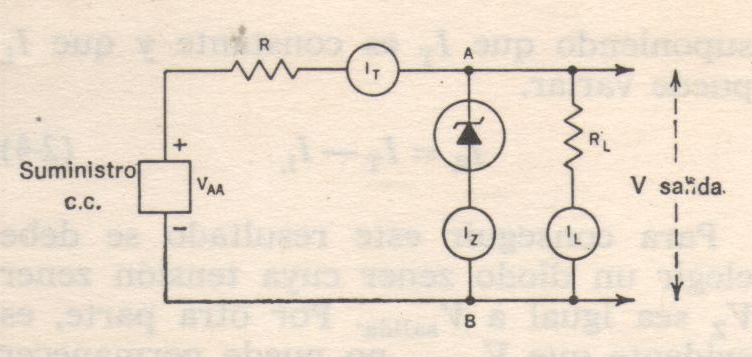
\includegraphics[width=0.6\textwidth]{regulador_shunt.png}
    \caption{Diodo zener utilizado como regulador shunt de tensión.}
    \label{fig:regulador_shunt}
\end{figure}

NOTA: En el análisis del circuito de la figura~\ref{fig:regulador_shunt}, que contiene elementos lineales (resistores) y no lineales (diodos zener), son aplicables las leyes de Ohm y Kirchhoff, lo mismo que las ecuaciones de redes que Ud. ya conoce.

Consideremos en primer lugar el funcionamiento del circuito cuando la tensión de la fuente $V_{AA}$ es constante, pero la corriente de carga $I_L$ cambia. Supongamos que se requiera una tensión de salida constante $V_{\text{salida}}$ entre los terminales de la carga. Las dos corrientes $I_L = V_{\text{salida}}/R_L$ e $I_Z = V_{\text{salida}}/R_Z$ se combinan formando la corriente total $I_T$; es decir,
\begin{equation}
    I_T = I_L + I_Z
\end{equation}
La tensión $V_R$ en los terminales de R es igual al producto de $I_T$ y R. Así pues
\begin{equation}
    V_R = I_T \times R
\end{equation}
pero
\begin{equation}
    V_{AA} = V_R + V_{\text{salida}}
\end{equation}
Por tanto, si $V_{AA}$ permanece constante y es necesario que $V_{\text{salida}}$ permanezca constante, $V_R$ debe mantenerse constante. Por consiguiente la corriente total $I_T$ debe permanecer invariable a pesar de las variaciones de la corriente de carga. Esto sólo se puede conseguir compensando las variaciones en $I_L$. O sea, $I_Z$ debe cambiar de la manera indicada por la ecuación (2-4)
\begin{equation}
    I_Z = I_T - I_L
\end{equation}
suponiendo que $I_T$ es constante y que $I_L$ puede variar.

Para conseguir este resultado se debe elegir un diodo zener cuya tensión zener $V_Z$ sea igual a $V_{\text{salida}}$. Por otra parte, es evidente que $V_{\text{salida}}$ no puede permanecer absolutamente constante. Debe variar lo suficiente para producir cambios de la corriente del diodo $I_Z$ que compensen los cambios de la corriente de carga $I_L$. Se debe elegir, pues, un diodo zener cuyas características de tensión y corriente satisfagan los requisitos del circuito. Además, este diodo debe funcionar en el punto correcto de su característica.

También se puede utilizar el diodo en la figura~\ref{fig:regulador_shunt} para compensar las variaciones de la tensión c.c. de alimentación cuando el resistor de carga $R_L$ permanece constante, asegurándose así una tensión de salida constante $V_{\text{salida}}$ y por tanto, una corriente de carga constante $I_L$. Supongamos que el circuito esté funcionando correctamente con un nivel de tensión c.c. $V_{AA}$. Si ahora se aumenta la tensión $V_{AA}$ de alimentación, la tensión de salida $V_{\text{salida}}$ tenderá a aumentar. En consecuencia, la corriente zener $I_Z$ aumentará, e $I_T$ aumentará asimismo cuanto disminuya la tensión $V_R$ entre los terminales de R. Si el circuito regulador ha sido correctamente diseñado, el aumento de la tensión entre los extremos de R, $\Delta V_R$, debe ser igual (aproximadamente) al incremento de la tensión de alimentación $\Delta V_{AA}$, y $V_{\text{salida}}$ volverá a tener su valor original. Análogamente, una disminución de $V_{AA}$ originará una disminución de $I_Z$ y, por tanto, de $I_T$. $V_R$ se reducirá y $V_{\text{salida}}$ volverá a tener su nivel predeterminado.

El valor de R elegido para conseguir la regulación correcta dependerá de las características del diodo y de las condiciones de variación de $V_{AA}$ e $I_L$.

Además del diodo regulador cuyo funcionamiento acabamos de describir, existen diodos de referencia de tensión cuya tensión zener es tan estable que se pueden utilizar como patrón de laboratorio o como tensión de referencia en un circuito regulador de tensión más complicado.

\subsection*{Consideraciones de diseño}
Un valor de diseño para R y para el diodo zener se puede calcular por los requisitos del circuito.

Supongamos que se requiera una tensión de salida $V_{\text{salida}}$ constante de 10 V ($\pm$ 0,7 V) para una carga cuya corriente $I_L$ pueda variar entre 5 y 20 mA. La potencia es suministrada al circuito desde una fuente de c.c. constante de 20 V. Se necesita diseñar un circuito de regulación para conseguir esto.

Supongamos un circuito regulador, tal como el representado en la figura~\ref{fig:regulador_shunt}, que satisface las especificaciones del problema. Debemos seleccionar un diodo zener regulador cuya $V_Z = 10$ V. Supongamos que es asequible un diodo que deje pasar una corriente de regulación $I_Z$ tal que la corriente total del circuito $I_T$ permanece constante en 30 mA en el margen de variación de la corriente de carga de nuestro problema. Por la ley de tensión de Kirchhoff podemos escribir
\begin{equation}
    V_{AA} = I_T \times R + V_{\text{salida}}
\end{equation}
y
\begin{equation}
    R = \frac{V_{AA} - V_{\text{salida}}}{I_T}
\end{equation}
Sustituyendo en la ecuación (2-6) los valores dados $V_{AA} = 20$, $V_{\text{salida}} = 10$, e $I_T = 30 \times 10^{-3}$ A, obtenemos
\[ R = \frac{20 - 10}{30 \times 10^{-3}} = 333 \, \Omega \]
Para determinar la potencia de R, observemos que hay una caída de 10 V en él. Por tanto
\[ W = \frac{V^2}{R} = \frac{10^2}{333} \approx \frac{1}{3} \, \text{W} \]
Una buena práctica de ingeniería requiere que el resistor esté sobredimensionado. Por tanto, se debe utilizar un resistor de 1 W 330 $\Omega$ $\pm$ 5 por 100.

La potencia del diodo se determina por la máxima corriente $I_Z$ que requiere el circuito. En nuestro problema la máxima $I_Z$ es 25 mA (cuando $I_L = 5$ mA). Pero la mínima potencia $W_Z$ es
\begin{equation}
    W_Z = V_Z \times I_Z = 10 \times 25 \times 10^{-3} = 250 \, \text{mW}
\end{equation}
Nuevamente la buena práctica de ingeniería requiere sobredimensionado el diodo y será suficiente uno de 500 mW.

\newpage
\section*{Resumen}
\begin{enumerate}
    \item Un diodo zener es un semiconductor cuya característica inversa tensión-corriente se utiliza en algunas aplicaciones de circuito electrónico.
    \item Un diodo zener mantiene una tensión constante $V_Z$ en su salida si está polarizado inversamente y funciona dentro de sus características nominales o especificadas.
    \item Cuando el diodo funciona con su tensión zener $V_Z$, pequeñas variaciones de la tensión en los terminales del diodo originan cambios de corriente relativamente grandes $I_Z$ en el diodo.
    \item Los diodos zener están especificados en cuanto: a) tensión zener $V_Z$; b) margen de tolerancia de $V_Z$; c) límites de corriente zener; d) máxima disipación de potencia, y e) máxima temperatura de trabajo.
    \item Se fabrican diodos zener que entregan tensiones desde uno hasta varios centenares de voltios.
    \item Los diodos zener se utilizan como reguladores de tensión y como patrones de referencia de tensión.
    \item Un regulador de tensión shunt correctamente diseñado (fig. 2-3) mantiene una tensión de salida constante $V_Z$ entre los terminales del diodo, a pesar de variaciones especificadas de la tensión de su entrada o cambios también especificados de la corriente de carga.
    \item En el regulador shunt de la figura~\ref{fig:regulador_shunt}, dada una tensión constante de alimentación $V_{AA}$, el diodo zener mantiene una corriente constante del circuito $I_T$, a pesar de las variaciones de la corriente de carga $I_L$. Así pues, si $I_L$ disminuye, $I_Z$ aumenta, y viceversa. En cualquier caso, para cambios especificados de $I_L$, la corriente zener $I_Z = I_T - I_L$.
    \item En el regulador shunt de la figura~\ref{fig:regulador_shunt}, si la corriente de carga permanece constante, pero la tensión de alimentación $V_{AA}$ aumenta, entonces $I_Z$ aumenta, aumentando $I_T$ y la caída de tensión en R, para mantener una tensión constante $V_{\text{salida}}$ entre los terminales del zener. Las tensiones satisfacen la ecuación $V_{\text{salida}} = V_{AA} - I_T \times R$. Análogamente, una disminución de $V_{AA}$ dará por resultado una disminución de $I_Z$ y por tanto de $I_T$. La caída de tensión en R igual a $I_T \times R$, disminuirá, manteniendo así una tensión constante de salida entre los terminales de la carga.
    \item En el regulador shunt de la figura~\ref{fig:regulador_shunt}, dadas $V_{AA}$, $I_T$, y $V_{\text{salida}}$, es posible calcular el valor de R por la fórmula
    \[ R = \frac{V_{AA} - V}{I_T} \]
\end{enumerate}

\begin{comment}
\section*{Autoexamen}
\begin{enumerate}
    \item Cuando se le utiliza como regulador de tensión, un diodo zener debe ser polarizado en sentido \underline{\hspace{1.5cm}} (directo/inverso).
    \item Si un fabricante especifica que para un zener la tensión de salida es 10 V $\pm$ 10\% de tolerancia, la $V_Z$ del diodo está comprendida entre \underline{\hspace{1cm}} V y \underline{\hspace{1cm}} V.
    \item La corriente en un diodo zener de 1 W 10 V debe ser limitada a un máximo de \underline{\hspace{1cm}} A.
    \item Un diodo zener de 20 V 1 W conectado como regulador de tensión en el circuito de la figura~\ref{fig:regulador_shunt} suministra una tensión de salida de \underline{\hspace{1cm}} V (aproximadamente) a la carga.
    \item En el circuito de la pregunta 4, la tensión c.c. de alimentación $V_{AA}$ es 30 V, e $I_L = 0,05$ A y es constante en un margen de corriente de carga de 5 a 35 mA. Dentro de este margen la corriente del diodo zener varía desde \underline{\hspace{1cm}} a \underline{\hspace{1cm}} mA.
    \item En el circuito de la pregunta 5, el valor de R que satisfará los requisitos del regulador es \underline{\hspace{1cm}} $\Omega$.
\end{enumerate}
\end{comment}

\section*{Materiales Necesarios}
\begin{itemize}
    \item Fuente de alimentación: Fuente de c.c. variable regulada.
    \item Equipo: EVM; VOM; miliamperímetro.
    \item Resistores: 1/2 W 3300 $\Omega$; 5 W 500 $\Omega$; resistores necesarios para el procedimiento adicional.
    \item Semiconductores: Diodo zener, 10 V 1 W.
    \item Diversos: Interruptor unipolar, caja de décadas de resistencias para pregunta adicional.
\end{itemize}

\newpage
\section*{Procedimiento}

\subsection*{Característica tensión-corriente. Polarización inversa}

\begin{figure}[H]
    \centering
    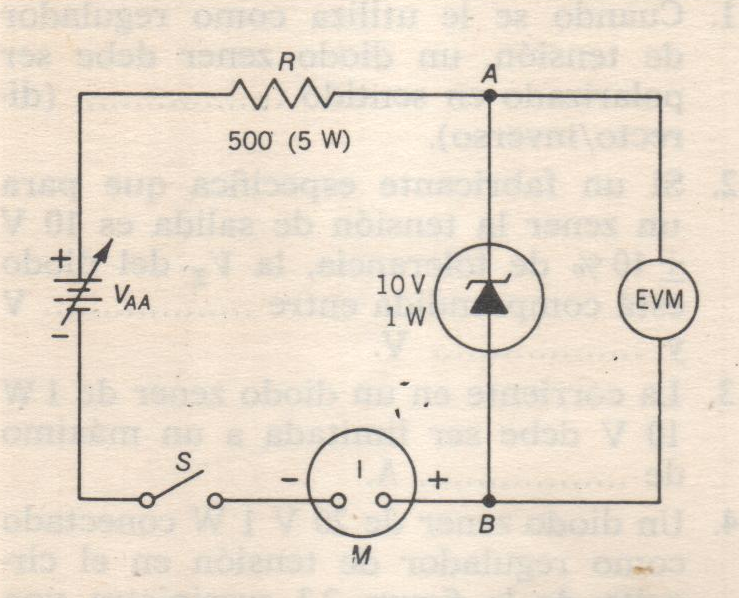
\includegraphics[width=0.6\textwidth]{circuito_inversa.png}
    \caption{Circuito experimental para observar el efecto de la polarización inversa sobre un diodo zener.}
    \label{fig:circuito_inversa}
\end{figure}

\begin{enumerate}
    \item Conectar el circuito de la figura~\ref{fig:circuito_inversa}. El interruptor S está abierto. $V_{AA}$ es una fuente de alimentación regulada ajustada en 0 V. M es un VOM 20.000 $\Omega$/V conmutado en el alcance más bajo de corriente.
    \item Cerrar S. Medir la corriente I del diodo, si la hay, con $V_{AA}$ ajustado en 0 V. Anotar los resultados en la tabla 2-1.
    \item Ajustar la salida de $V_{AA}$ para que la tensión $V_{AB}$ medida entre los terminales del diodo sea 2,0 V. Medir la corriente I del diodo. Anotar los resultados en la tabla 2-1. Repetir las operaciones del apartado 3 para cada valor de $V_{AB}$ indicado en la tabla 2-1. Cambiar el alcance de M como se requiera. Calcular la resistencia $R_Z$ del diodo ($R_Z = V_{AB}/I$) y anotar los resultados en la tabla 2-1.
    \item Ajustar la salida de $V_{AA}$ para que la corriente I del diodo mida 2 mA. Medir la tensión $V_{AB}$ entre los terminales del diodo y anotarla en la tabla 2-1. Calcular $R_Z$ y anotarla en la tabla 2-1.
    \item Repetir el apartado 4 para cada valor de la corriente indicado y anotar los valores correspondientes de $V_{AB}$ y $R_Z$ en la tabla 2-1.
\end{enumerate}

\begin{table}[H]
    \centering
    \caption{Polarización inversa.}
    \label{tab:pol_inversa}
    \begin{tabular}{ccc|ccc}
        \toprule
        $V_{AB}$, V & $I$, mA & $R_Z$, $\Omega$ & $V_{AB}$, V & $I$, mA & $R_Z$, $\Omega$ \\
        \midrule
        0 & & & & 5 & \\
        2,0 & & & & 10 & \\
        6,0 & & & & 20 & \\
        7,0 & & & & 30 & \\
        8,0 & & & & 40 & \\
        & 2 & & & 50 & \\
        \bottomrule
    \end{tabular}
\end{table}

\subsection*{Característica tensión-corriente. Polarización directa}
\begin{enumerate}[resume]
    \item Abrir S, desconectando la potencia del circuito. Ajustar la salida en la fuente de alimentación en 0 V. Invertir el diodo en el circuito.
    \item Cerrar S. Medir y anotar en la tabla 2-2 la corriente directa en el diodo en cada nivel de tensión $V_{AB}$ indicado en la tabla. Calcular la resistencia directa $R_F = V_{AB}/I$. Anotar los resultados en la tabla 2-2.
    \item 
    \begin{enumerate}[label=\alph*)]
        \item Por los datos de las tablas 2-1 y 2-2 dibujar un gráfico de la corriente del diodo (eje vertical) en función de la tensión del diodo.
        \item Dibujar un gráfico ampliado de la corriente del diodo en función de la tensión en la región zener.
        \item Dibujar gráficos separados de la resistencia del diodo en función de la tensión para las disposiciones de polarización inversa y polarización directa.
    \end{enumerate}
\end{enumerate}

\begin{table}[H]
    \centering
    \caption{Polarización directa.}
    \label{tab:pol_directa}
    \begin{tabular}{lcccccccccc}
        \toprule
        $V_{AB}$, V & 0 & 0,1 & 0,2 & 0,3 & 0,4 & 0,5 & 0,55 & 0,6 & 0,65 & 0,7 \\
        \midrule
        $I$, mA & & & & & & & & & & \\
        $R_F$, $\Omega$ & & & & & & & & & & \\
        \bottomrule
    \end{tabular}
\end{table}

\subsection*{El diodo zener como regulador de tensión}

\begin{figure}[H]
    \centering
    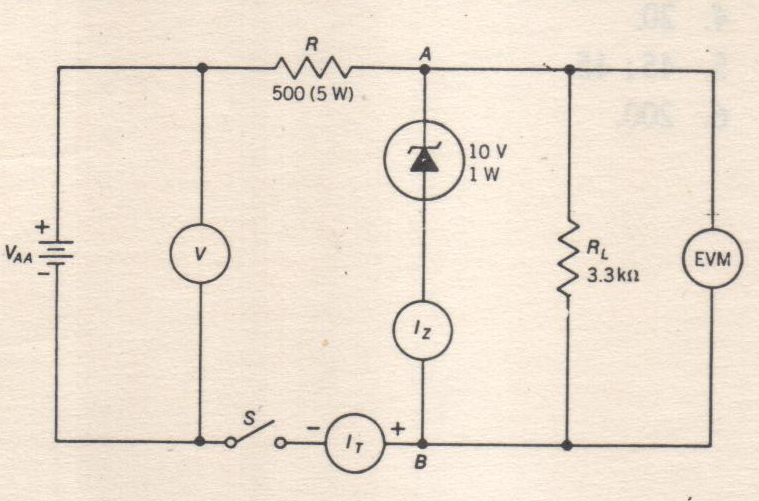
\includegraphics[width=0.6\textwidth]{circuito_regulador.png}
    \caption{Circuito experimental de regulador de tensión.}
    \label{fig:circuito_regulador}
\end{figure}

\begin{enumerate}[resume]
    \item Conectar el circuito de la figura~\ref{fig:circuito_regulador}. El interruptor S está abierto. La salida de la fuente de alimentación $V_{AA}$ se ajusta a 0 V. M es un miliamperímetro conmutado en el alcance de 100 mA.
    \item Cerrar S. Aumentar lentamente la tensión de alimentación $V_{AA}$ hasta que la corriente $I_Z$ existente en el diodo mida 20 mA. Medir la tensión de alimentación $V_{AA}$ y la tensión $V_{AB}$ entre los terminales de la carga. Anotar los resultados en la tabla 2-3. Medir la corriente total $I_T$. Anotar los resultados en la tabla 2-3.
    \item Determinar y anotar el margen de variación de $V_{AA}$ en el cual $V_{AB}$ permanece constante dentro de $\pm$ 0,1 V de su valor en el apartado 8. Medir la variación de $I_Z$ y la de $I_T$ dentro de la de este margen. Anotar los resultados en la tabla 2-3.
\end{enumerate}

\begin{table}[H]
    \centering
    \caption{Regulación de tensión.}
    \label{tab:regulacion}
    \begin{tabular}{cccc}
        \toprule
        $V_{AB}$, V & $I_Z$, mA & $I_T$, mA & $V_{AA}$, V \\
        \midrule
        $V_{AB}$ & 20 & & \\
        $V_{AB} + 0,1$ & & & \\
        $V_{AB} - 0,1$ & & & \\
        \bottomrule
    \end{tabular}
\end{table}

\subsection*{Adicional (opcional)}
\begin{enumerate}[resume]
    \item 
    \begin{enumerate}[label=\alph*)]
        \item Diseñar un circuito regulador de una fuente de tensión constante $V_{AA}$, utilizando el diodo zener cuya característica tensión-corriente acaba Ud. de determinar experimentalmente. Se pide que el regulador mantenga una tensión constante de salida $V_{\text{salida}}$ dentro de 0,2 V del valor medio de $V_{\text{salida}}$, para corrientes de carga comprendidas en el margen de 10 a 30 mA. Dibujar el circuito indicando los valores de los componentes y de las tensiones. Explique Ud. cómo ha determinado estos valores.
        \item Probar el circuito y anotar los resultados de las mediciones en la tabla 2-4. Utilizar una caja de décadas de resistencia como carga variable.
    \end{enumerate}
    \item Graficar las curvas y observar la característica tensión-corriente del diodo zener. Dibujar la curva en el mismo papel gráfico que en el apartado 8.
\end{enumerate}

\begin{table}[H]
    \centering
    \caption{Características del diseño del regulador de tensión.}
    \label{tab:diseno_regulador}
    \begin{tabular}{ccccc}
        \toprule
        $V_{AA}$, voltios & R, ohmios & $I_L$, mA & $R_L$, ohmios & $V_{\text{salida}}$, voltios \\
        \midrule
         & & 5 & & \\
         & & 10 & & \\
         & & 15 & & \\
         & & 20 & & \\
         & & 25 & & \\
        \bottomrule
    \end{tabular}
\end{table}

\newpage
\section*{Preguntas para el Informe}
\begin{enumerate}
    \item Comparar la polarización de un diodo de unión (Práctica 1) con la de un diodo zener en una aplicación normal.
    \item Comparar la característica tensión-corriente del gráfico del diodo zener del apartado 8a de esta Práctica con la característica representada en la figura~\ref{fig:caracteristica_zener}. Explicar las diferencias que haya.
    \item ¿Qué porción de la característica de un diodo zener es más útil en las aplicaciones del regulador de tensión? ¿Por qué?
    \item a) ¿Cuál es el significado del gráfico obtenido en el apartado 8b? b) ¿Cómo se puede utilizar el gráfico obtenido en el apartado 8b para diseñar un regulador empleando un diodo zener de 10 V?
    \item Referencia a la tabla 2-3. Explicar cómo funciona este circuito regulador.
    \item[6.] \textbf{(Adicional (opcional))} Explicar el funcionamiento del circuito regulador que ha diseñado Ud. en el apartado 12.
    \item[7.] \textbf{(Adicional (opcional))} ¿Compensará el circuito regulador de la figura~\ref{fig:circuito_regulador} las variaciones de la tensión de entrada $V_{AA}$ y las variaciones de la corriente de carga $I_L$? Explicarlo.
\end{enumerate}

\begin{comment}
\section*{Respuestas a las preguntas de autoexamen}
\begin{enumerate}
    \item Inverso.
    \item 9; 11.
    \item 0,1.
    \item 20.
    \item 45; 15.
    \item 200.
\end{enumerate}
\end{comment}

\end{document}